%
% Annual Cognitive Science Conference
% Sample LaTeX Paper -- Proceedings Format
%

% Original : Ashwin Ram (ashwin@cc.gatech.edu)       04/01/1994
% Modified : Johanna Moore (jmoore@cs.pitt.edu)      03/17/1995
% Modified : David Noelle (noelle@ucsd.edu)          03/15/1996
% Modified : Pat Langley (langley@cs.stanford.edu)   01/26/1997
% Latex2e corrections by Ramin Charles Nakisa        01/28/1997
% Modified : Tina Eliassi-Rad (eliassi@cs.wisc.edu)  01/31/1998
% Modified : Trisha Yannuzzi (trisha@ircs.upenn.edu) 12/28/1999 (in process)
% Modified : Mary Ellen Foster (M.E.Foster@ed.ac.uk) 12/11/2000
% Modified : Ken Forbus                              01/23/2004
% Modified : Eli M. Silk (esilk@pitt.edu)            05/24/2005
% Modified: Niels Taatgen (taatgen@cmu.edu) 10/24/2006

%% Change ``a4paper'' in the following line to ``letterpaper'' if you are
%% producing a letter-format document.

\documentclass[10pt,letterpaper]{article}
\setlength{\belowcaptionskip}{5pt plus 3pt minus 2pt}
\usepackage{cogsci}
\usepackage{graphicx}
\usepackage{amsmath, amsthm, amssymb}
\usepackage{pslatex}
\usepackage{apacite}
\usepackage{multirow}
\usepackage{arydshln}
\usepackage{soul,color}
\usepackage{xspace}
%\usepackage[natbib=true]{biblatex}
\usepackage{natbib}
\usepackage{textcomp}
\usepackage[font = small]{caption}
\setlength{\belowcaptionskip}{-7pt}
\def\bibfont{\small}

\title{Present bias in exploratory choice}

\author{  {\large \bf Alexander S. Rich (asr443@nyu.edu)} \\ {\large\bf Todd M. Gureckis (todd.gureckis@nyu.edu)}\\
        New York University, Department of Psychology, 6 Washington Place, New York, NY 10003 USA}
\begin{document}
\maketitle

\begin{abstract}

  \textbf{Keywords} time preference, present bias, exploratory choice
\end{abstract}

The problem of under-exploration seems remarkably common. One of the most severe
expressions of under-exploration is learned helplessness, in which an organism
experiences the absence of contol over the environment, learns that the
environment is uncontrollable, and thus ceases to take actions that might allow
it to regain its sense of control. Learned helplessness has been proposed to
underly most notably depression\cite{Abramson1978, Abramson1989} but also
problems ranging from difficulties in school CITE to poverty CITE.

While the cognitive appraisal of experienced events affects the development of
learned helplessness \citep{Abramson1978}, patterns of exploration clearly play
a role as well \citep{Huys2009, Teodorescu2014a}. In the case of depression,
interventions aimed at increasing the exploration of activities this might
produce a sense of pleasure and mastery have been found to be as effective as
those with a more cognitive orientation \citep{Jacobson1996}.

Under-exploration also seems to occur in the development of complex skills, such
as flying a plane or playing a sport CITE. In these settings, an ``emphasis
change'' training method in which the focus of practice is repeatedly changed
can lead to greater performance gains than unguided practice or more complex
training methods. Emphasis change works because it encourages people to
continually explore the performance space to find more effective cognitive and
motor routines CITE. Without these interventions, people often enter a ``local
maximum'' in which exploration decreases and performance plateaus CITE.

There are many other areas in which under-exploration is less clearly
established, but is suspected to play a role in maladaptive behavior.
Insufficient exploratory interaction with outgroups may be one cause of
stereotypes and prejudice \citep{Denrell2005most}, and interventions that
increase inter-group contact reduce stereotypes \citep{Shook2008}. The crowding
out of exploration by exploitation is a concern in organizational behavior as
well\cite{March1991, Levinthal1993}, prompting research into organizational
structures that may preserve exploration \citep{Fang2010}.

\subsection{Under- and over-exploration in the lab}

Given the seeming pervasiveness of under-exploration in real-world decision
making, one might expect a clear pattern of under-exploration in lab
experiments. Instead, however, lab results are mixed, with people sometimes
under-exploring, sometimes over-exploring, and sometimes exploring close to an
optimal amount. To take two illustrative examples, \citet{Zwick2003} found that
in a sequential search task people under-searched when there were no information
costs but over-searched when there were information costs, and
\citet{Teodorescu2014} found that people explored unknown alternatives too often
or not often enough depending on whether rare outcomes were positive or
negative. Similar results have been obtained within and across a variety of
other studies and paradigms
\citep{tversky1966information, Busemeyer1988, hertwig2004decisions, Navarro2016, Juni2016, Sang2011}.

These experimental studies raise the question of why under-exploration appears
more widespread than over-exploration in the field, but not in the lab. One
possibility is that both forms of deviation from optimality are in fact
prevalent, though perhaps in different settings, and that the seemingly general bias
toward under-exploration is illusory. However, in the current paper we propose
instead that lab tests of exploratory choice have been missing a key component
of real-world exploratory choice, namely, the distribution of choices and
outcomes over time, and that this spreading of exploratory choices over time may
account for the tendency to under-explore.

% In ``observe or bet'' tasks in which people choose to either
% obtain information or reward on each trial, people appear to collect much more
% information than is needed \citep{tversky1966information}. But, in settings
% where the underlying reward probabilities might change, information-seeking
% appears close to optimal \citep{Navarro2016}.

\subsection{Exploration and myopia}

Under-exploration is often proposed to be the result of myopia: the
underweighting of temporally distant rewards relative to close ones \cite{March1991, Levinthal1993}. While
choosing actions that are expected to immediately maximize reward is inherently
exploitative, exploration often requires the decision-maker to suffer short-term
costs in search of better future options.

There are two distinct possible causes of myopia \citep{Bartels2015}. The first is that the decision-maker is
unaware of or fails to consider the future. This form of myopia is likely one
cause of under-exploration, particularly in complex environments. However,
researchers in exploratory choice have begun to address this form of myopia, and
have found that people change their
patterns of exploration based on their expectations about future choices,
showing that, at least to some degree they do consider the future \citep{Meyer1995, Wilson2014a, Rich2017}.

The the second form of myopia is that the decision-maker
is aware of the future but simply doesn't care as much about it.
A wealth have studies have shown that this form of myopia is an important factor
in human decision making, and that people are strongly
biased towards present . For example, people will often prefer a larger, later monetary
reward to a smaller, sooner reward when both rewards are in the future. But when the
time until both rewards is reduced so that the sooner reward is immediate, the
sooner reward seems to loom larger and
people may switch their preference \citep{Kirby1995}. With non-monetary rewards,
such as the cessation of an annoying noise \citep{Solnick1980}, watching a video
when bored \citep{Navarick1998}, or drinking soda
when thirsty \citep{Brown2009}, a bias towards immediate rewards has been observed on the scale of
minutes or even seconds.

Present bias has the clear potential to cause people to explore too little, by
increasing the perceived immediate gains of exploiting relative to the delayed
gains of exploring. However, to date there has been no experimental research
examining how people's bias towards the present affects exploratory choice. In
part, this is a product of limits in experiment design. In most exploratory
choice experiments, each choice and outcome takes fewer than 10 seconds to
complete, making it unlikely for a large bias to develop between the current
trial and future ones. More importantly, regardless of the length of each trial,
rewards are generally not consumed on a trial-by-trial basis. For example, a participant
might recieve ``points'' on each trial, which are converted to money when the
experiment ends. In this sort of paradigm, there is no reason to expect a bias
towards the present choice's rewards over future rewards, as all rewards are
infact delivered at the same time.

In the present study, we seek to address the lack of research on present bias
and exploratory choice. We develop a novel exploratory choice task using
real consumption rewards, and compare behavior when the outcome of each
choice is consumed immediately to behavior when outcomes are temporally delayed.

% why? underexploration is often proposed to be the result of myopia;
% overweighting of the present relative to the future.
% - exploration benefits future, exploitation benefits present.
% - two meanings of myopia (Bartels); one is unaware of the future, or fail to
% consider future, second is aware of the future but simply don't care about it as much.
% - simple adaptive models often exhibit first kind of myopia, and consequently
% underexplore. But experimental studies show that, at least in some cases, people
% are cognizant of the future and adjust their exploration based on it. So unclear
% that unawareness of future is major driver of under-exploration
% - But the second type of myopia, not caring about the future, appears to be very
% common in people. People seems to be present biased

% - this present bias hasn't been studied in exploratory decision making. Most
% studies take place over a short amount of time, such that there are only a few
% seconds dividing the present choice from future choices. Also crucially, rewards
% are usually a medium such as ``points'' that are not consumed immediately, but
% are converted to money all at once at the end of the experiment. Thus present
% and future choices all yield reward at the same time, so a bias towards present
% rewards will likely have no effect on behavior.

% - alternative is that even though exploratory choices contain a present-future
% trade-off, people don't treat them that way, and exploration is driven by things
% like ``exploration bonuses'' that aren't sensitive to time.

\section{Experiment}

\begin{figure*}[htp]
\centering
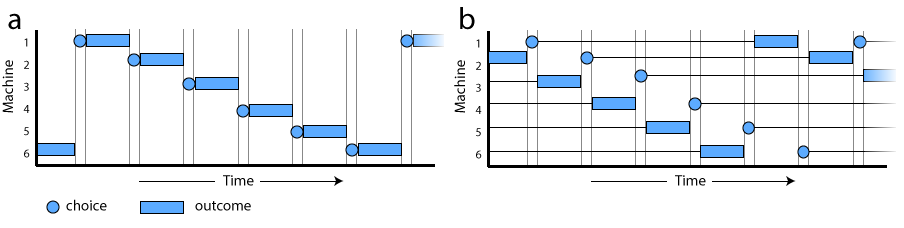
\includegraphics[width=\textwidth]{figures/machinetimeline.png}
\caption{A schematic illustration of the two conditions. In both conditions, six
30-second work periods pass between consecutive choices with a given machine. In
the immediate condition (left), the outcome for a choice is revealed and occurs immediately after the
choice is made. In the delayed condition (right), the outcome of a choice is revealed
and occurs after a delay of four work periods.}
\label{fig:machinetimeline}
\end{figure*}

\subsection{Method}

\subsubsection{Participants.}

\subsubsection{Design and procedure.}

Participants were informed that their job was to perform a monotonous slider task that
would be split into 30-second ``work periods'', but that they would be able to
make choices throughout the experiment that would give them a chance to watch a
Youtube video instead. The number of remaining work periods in the experiment was shown
at the top of the screen, as was the number of seconds left in the current work period.

The slider task was based of a task previously used by \citet{Gill2012}. In each
period of the slider task, five horizontal sliders appeared on the screen. Each
started at a random setting between 0 and 100, with the slider's value
shown to its right, with a random horizontal offset so that the
sliders were not aligned. The participant's task was to use the mouse to move
each slider to ``50'' before the work period ended. When a participant released
the mouse at the correct setting, the slider turned green to show it had been
completed. To ensure that the task took close to the allotted 30 seconds, at the
beginning of the task only the top slider was enabled, and the other four were
grayed out. Additional sliders were enabled at five-second intervals, such that
all five sliders were available after 20 seconds.

Before beginning the experiment, participants chose one of four videos available
on Youtube: an episode of ``Planet Earth'', and episode of ``The Great British
Bakeoff'', and episode of ``Mythbusters'', or an Ellen Degeneres comedy special.
The video was embedded in the experiment with all user controls (such as
skipping ahead) disabled. When given access to the video, participants had to keep the
browser window open and hold down the space bar for the video to play. This allowed us to ensure that
participants maintained engagement with the content.

In the main part of the experiment, participants completed a total of 70 work
periods. For the first 10 (in the immediate condition) or 6 (in the delayed
condition) work periods, participants simply clicked a button to begin the
slider task. After these initial periods, participants gained access to six
``machines'', each of which had a ``current spinner'' and a ``new spinner''.
Before each work period, participants clicked the circled machine,
were shown the machine and made a choice about which spinner to run. Based on their choices, there was a
chance the machine would perform the work task for the participant, allowing the
participant to watch their chosen video instead.

In the immediate condition, the machine ran immediately after the choice was
made, and affected the next work period. It then ``cooled off'' for the
following five periods, as choices were made with the other five machines.

In the delayed condition, the machine had to ``process'' for four work periods
after a choice was made, thus delaying the outcome by least 2 minutes.
The participant then clicked the machine again to
return to it and observe its outcome, and either perform the slider task or
watch the video. The machine then cooled off for a single period before being ready
for another choice. In the first four periods in which machines were available
in the delayed condition, participants made a choice but then simply pressed a
button to begin the slider task (as no machine had yet finished processing). In
the final four periods, participants observed the outcomes of the machines but
made no more choices.

At each choice, participants had to select between two options: run the
machine's ``current spinner'' or run a ``new spinner''. Each machine had two
circular spinners with arrows at the top. The current spinner was split into
five black and five gold wedges. If a participant chose the
current spinner, it spun (immediately or after four periods, depending
on the condition) and, if the arrow landed on the gold wedge, the machine
worked and the participant could watch the video. Initially, the
current spinner's gold wedges were randomly set for each machine to cover between
1/3 and 2/3 of the spinner.

The new spinner initially showed a question mark. If a participant chose the
new spinner, then (immediately or after four periods) a new spinner was
created and appeared on the machine. The new spinner's gold wedges could cover
anywhere from 0\% of the spinner to 100\% of the spinner. The new spinner then
spun and, if the arrow landed on a gold wedge, the machine worked.
Additionally, if the new spinner had a greater gold area than the current
spinner, the new spinner was ``saved'' and the current spinner was
updated to the new spinner.  This meant that
while choosing a new spinner carried some risk, it also carried long-term
benefits as the current spinner could be improved from its initial value.

Finally, in order to induce exploration throughout the entire experiment, the
six machines would occasionally ``reset'' after they ran. When this occured, a
the current spinner would be set to a new random value between 1/3 and 2/3 gold.
Participants were informed that this would occur randomly on
1/6 of trials. In fact, the procedure was designed so exactly one of the six
machines would reset on each cycle through the machines, and no machine would be
reset on two consecutive uses.

During the machine choices, participants had access to an ``info'' button at the
bottom of the screen that provided reminders about the dynamics of the task. In
addition, before beginning the full experiment, participants completed two
practice phase. First, they performed several trials of practice using the
machines, with the actual work periods removed. Then, they performed three work
periods practicing the slider task.

Participants were given a performance-based bonus of \$3.00 for completing the
slider tasks accurately. If they missed fewer than 10\% of sliders throughout
the experiment and left the video paused less than 20\% of the time, they were
not penalized. However, if they missed more sliders or left the video paused for
longer, they lose 10 cents from their bonus for each additional percentage of
sliders missed or time with the video paused. The running percentage of sliders
missed and video pause time was displayed at the top of the screen throughout
the experiment.


% People often choose actions based not on full information
% about the possible outcomes, but rather on their own past experiences
% \citep{hertwig2004decisions, hertwig2009description}. Making decisions
% from experience is necessary in an uncertain and changing environment,
% but it can cause persistent biases because current beliefs
% and choices can prevent the collection of information that would
% improve future choices. One of the most fundamental biases of
% experience-based decision-making is what \citet{denrell2001adaptation}
% called the ``hot stove effect,'' in which a negative experience with a
% prospect causes an agent to avoid that prospect in the future, preventing
% further belief revision~\citep{denrell2001adaptation,
%   denrell2007adaptive}.  For example, suppose you attend a weekly
% lecture series for the first time and, while the series is usually
% good, you happen to attend a boring talk. This negative experience
% might stop you from attending the series in the future, and as a
% result you might persistently believe the lecture series is boring and
% not attend. This type of false belief can't as easily develop in the
% positive domain; if a lecture series is usually boring but you happen
% to attend a stand-out talk, you're likely to keep attending future
% talks and will soon learn the truth.
% This potential to form false but persistent negative beliefs about
% stochastic prospects, and thus avoid them, has been proposed as a
% possible explanation of risk- and novelty-aversion by people, animals,
% and organizations in a wide variety of contexts
% \citep{denrell2007adaptive, denrell2005most,
%   niv2002evolution}.  
  

% %    
% The hot stove effect is a \emph{learning trap}---a robust
% sub-optimality which follows as a consequence of the incremental
% nature of belief revision \citep{Erev2014}.  In the current paper, we
% describe how the process of selective attention during category
% learning can exacerbate this learning trap, present experimental
% evidence of this bias, and finally propose interventions that may help
% decision makers escape it.

% %The hot stove effect is most typically discussed in the context of
% %``approach-avoid'' decisions, where an agent must repeatedly choose
% %whether to approach an uncertain prospect 
 


% \subsection{Attention and the Hot Stove Effect}

% Past work has focused on the hot stove effect as a problem emerging
% from experience-based decisions about a single stochastic
% prospect which sometimes yields negative outcomes. But real-world 
% environments are more richly structured, with a wide variety of prospects 
% related in complex ways. Rather than mitigate choice biases, such complexity
% may make them worse in ways not considered in past work. We theorize
% that in a complex environment, a pronounced ``attentional'' hot stove
% effect can emerge, even if outcomes are completely deterministic,
% due to people's tendency to categorize the environment based on a low
% number of dimensions or features.

% Most major theories of categorization \citep[e.g.,][]{Nosofsky1986a,
%  love2004sustain} posit that people learn to selectively
% allocate their attention to features that best discriminate category
% members. This conjecture is supported by findings that
% category structures with fewer relevant features are easier to learn
% \citep{Shepard61learning, nosofsky1994comparing} and that people tend 
% to make eye movements only to relevant features \citep{Rehder2005}. 
% In most cases, selective
% attention supports optimal performance by magnifying differences
% between categories. But interestingly, it can also slow learning in
% some cases, particularly when a person learns to \emph{not} attend to
% a certain dimension that may be useful later. This has been observed
% in studies of blocking and backwards blocking \citep{Mackintosh1975,
%   Kruschke2000}, as well as experiments in which subjects were first
% trained on one category structure and then tasked with learning a
% second which involved previously-irrelevant dimensions
% \citep{Kruschke1996}.

% To see how selective attention can ``trap" learners into a persistent
% false belief, consider an environment where an agent encounters
% different prospects that possess or lack each of several features.  Prospects
% that are approached yield a deterministic positive or negative reward 
% but no outcome is experienced when a prospect is avoided.
% The agent's problem now is not just of estimating whether
% a single prospect's value is positive but also of categorization---that
% is, of determining which combinations of features signify that a
% prospect should be approached, and which signify it should be avoided.


% \begin{figure}[t]
% \centering
% \includegraphics[width=\columnwidth]{figures/selectiveattention.pdf}
% \caption{\emph{a:} An deterministic environment containing prospects
%   with two binary features, where only prospects possessing both
%   features are negative. By attending to both features, a
%   decision-maker can avoid all negative prospects while exploiting all
%   positive prospects. \emph{b:} Early experience happens to highlight
%   the relevance of Feature 1. \emph{c:} The agent begins to attend
%   only Feature 1, and ignore Feature 2, making items with and without
%   Feature 2 appear equivalent. Items without Feature 1 are positive,
%   while the value of items with Feature 1 appear stochastic. \emph{d:}
%   The agent now avoids items with Feature 1, since some are
%   negative. This prevents the agent from gaining feedback which would
%   cause it to change its behavior.}
% \label{fig:attention}
% \end{figure}

% Suppose that two features, Feature 1 and Feature 2, are relevant to a
% prospect's value, and only prospects with both features are negative,
% as shown schematically in Figure~\ref{fig:attention}a. As the agent
% begins to gain experience approaching negative prospects
% (Figure~\ref{fig:attention}b), it will likely learn that prospects
% with certain exact combinations of features are negative and should be
% avoided.  But interestingly, it might also try to learn \emph{which}
% of the features was relevant to it being negative.  If experience
% suggests Feature 1 is relevant, for example, it may hypothesize that
% Feature 1 is the sole relevant feature and attend more strongly to
% whether a prospect has Feature 1 in the future. If this tendency is
% extreme, the agent may ignore Feature 2 almost completely
% (Figure~\ref{fig:attention}c).


% If only one dimension is attended, a situation quite like the
% traditional hot stove effect develops. All prospects with Feature 1
% are avoided, including those that lack Feature 2, even though the
% agent had no negative experience with such prospects. What's more, the
% bias away from these prospects is persistent, since avoidance of
% prospects with Feature 1 prevents the agent from collecting the information
% which would cause it to modify its current hypothesis, as shown in
% Figure~\ref{fig:attention}d. The agent may indefinitely
% avoid positive regions of the environment, as well as hold false
% beliefs about how the environment may be divided into meaningful
% categories.


% \subsection{Model simulation}

% To quantitatively verify that biases of the kind described above could
% develop, and their connection to selective attention, we conducted
% several simulations using a version of the ALCOVE model of
% categorization \citep{Kruschke1992a}, modified for a reinforcement
% learning setting in which feedback is action-dependent
% \citep[see][]{Jones2010}. We tested the model on a four-feature
% category structure, where approaching prospects with both Features 1
% and 2 yielded a payoff of $-5$ and approaching any other prospect
% yielded a payoff of $1$. This environment matches the structure depicted in
% Figure~\ref{fig:attention}, but with two added irrelevant features. Simulations were run
% with a specificity constant $c = 6$, a temperature parameter
% $\phi = 15$, an output-weight learning rate $\lambda_w = 0.1$, and an
% attention learning rate $\lambda_\alpha = 0.1$.

% We ran the model for 15 blocks of 16 trials each, across five
% simulation conditions. In the \emph{contingent, att} condition, the
% model only received feedback on the value of a prospect when it
% approached.  In the \emph{full-info, att} condition, the model
% received feedback on the value of all prospects irrespective of
% approach decisions.  The \emph{contingent, no-att} and
% \emph{full-info, no-att} conditions mirrored the first two conditions
% but with the attention-learning parameter was set to zero.  Finally,
% in the \emph{random-info, att} condition the model was yoked to
% receive feedback on the same proportion of trials as the contingent
% model, but the feedback trials were randomly selected and independent
% of the model's choices. The results of these simulations are plotted
% in Figure~\ref{fig:model}.



% \begin{figure*}[htp]
% \centering
% \includegraphics[width=\textwidth]{figures/modelplot.pdf}
% \caption{ALCOVE model simulations of approach-avoid decision-making in
%   five attentional/informational conditions. \emph{Left:} average
%   score per block of 16 trials; \emph{Center:} proportion of positive
%   prospects approached; \emph{Right:} proportion of negative prospects
%   approached. A persistent learning bias develops only when the model
%   received action-dependent feedback and is endowed with selective
%   attention. All conditions were simulated for 1000 model runs.}
% \label{fig:model}
% \end{figure*}



% As depicted in the left-most panel, agents in the contingent
% condition  fell into the learning trap and developed a
% persistent bias, failing to reach perfect performance.  In contrast, 
% agents in the full-info condition quickly reached
% peak performance of 12 points per block. The $p(approach|good)$ and
% $p(approach|bad)$ plots (middle and right panel, respectively) show 
% that the lower performance of the contingent
% condition was not due to continued approach of negative, costly
% prospects, but rather due to the persistent avoidance of some positive
% prospects.

% When attention learning is removed, the persistent bias disappears and
% the model reaches near-peak performance by the last block, though it
% is slower to learn to avoid negative prospects. This should not be
% interpreted simply as evidence that selective attention is generally
% harmful in this environment. On the contrary, with full information,
% selective attention leads to better performance; the full-info,
% no-att condition performs poorly, overgeneralizing from the negative
% prospects. It is only when feedback is dependent on current belief and
% action that selective attention becomes a disadvantage.

% It is also not the case that the contingent condition is biased due
% to a general lack of information. In the random-info condition, where
% the model is given the same number of feedback experiences as the
% contingent condition but distributed evenly over the space of prospects, no
% bias develops. Thus, the attentional hot stove effect occurs due not to an overall
% poverty of information but to a specific pattern of behavior
% which prevents information from being gained about prospects which
% could correct the model's misallocated attention.

% Finally, it is worth noting that in our simulations we assume that
% nothing is encoded in the absence of feedback. However, recent
% experiments have suggested that people might employ constructivist
% coding in the absence of feedback, essentially storing the exemplar as
% though the expected outcome had occurred and reinforcing existing
% beliefs~\citep{henriksson2010coded}. With this
% coding scheme, we would expect the attentional hot stove effect
% exhibited by ALCOVE to be even more pronounced.

% \section{Experiment}

% To test the degree to which people are susceptible to the
% attentional hot stove effect, we performed a simple experiment similar
% to the category-learning task described above.

% \subsection{Method}

% \subsubsection{Participants.}
% One hundred one participants were recruited via Amazon Mechanical
% Turk. Participants received \$1.25 for participation and received a
% performance-based bonus that ranged up to \$1.80.

% \subsubsection{Stimuli.}
% Stimuli were computer-generated cartoon bees that varied on four
% binary dimensions; they had two or six legs, a striped or spotted
% body, single or double wings, and antennae or no antennae, for a total
% of 16 unique stimuli (Figure~\ref{fig:stim}). Two of the four
% dimensions were chosen as relevant, counterbalanced across
% participants. Of the four possible combinations of values on these two
% dimensions, one was chosen at random; stimuli with this combination of
% values were  ``dangerous,'' and the remaining stimuli were
% ``friendly.''


% \subsubsection{Procedure.}
% Participants played the role of a beekeeper collecting honey from
% several beehives. They were told that each hive contained a single
% variety of bees, and that while most hives contained friendly bees
% that would give them honey, some
% hives had been invaded by dangerous bees, which would sting them if
% they tried to harvest.

% In the learning phase, participants encountered each of the 16 bee
% varieties 4 times, for a total of 64 trials. They were informed of the
% number of trials, and a the number of remaining trails was displayed
% throughout learning. Stimuli were ordered such that
% every eight stimuli contained two dangerous and six friendly bee
% varieties, and were otherwise random. On each trial, participants
% visited a new beehive, and were shown one of the bees in the
% hive. Based on the bee's appearance, they then had to choose either to
% attempt to harvest honey from the bee variety in that hive or to avoid
% the hive. When participants chose to harvest, they received honey and
% added \$0.02 to their bonus if the bee variety was friendly, but were
% stung and lost \$0.10 from their bonus if it was dangerous. When
% participants chose to avoid a hive, they gained \$0.00.  Participants
% started the game with a bonus of \$0.40.

% Participants were split into two conditions, which differed in 
% the feedback received upon avoiding a beehive. In the contingent
% condition, no feedback was provided when a participant avoided
% a hive. In the full-info condition, participants still gained
% \$0.00 when they avoided a hive, but were informed of whether the bee
% variety was friendly or dangerous and of what their payoff would have
% been had they harvested.

% The learning phase was followed by a surprise test
% phase.  During the test phase, participants encountered each variety
% twice and chose to harvest or avoid hives as before, but received no
% feedback about the outcomes of their actions and were not able to see
% changes to their bonus. This phase provided a comparison of
% learning under equivalent conditions.

% After the test phase, participants were informed of their total
% bonus, and were asked two final questions: ``About what percentage of
% beehives do you think contained dangerous bees?'' and ``Which features
% do you think were useful in deciding whether a bee variety was
% friendly or dangerous?''. For the first question, participants entered
% a percentage between 0 and 100, and for the
% second question participants could choose any combination of the four
% features using check-boxes.

% \begin{figure}[htp]
% \centering
% \includegraphics[width=\columnwidth]{figures/stimuli.pdf}
% \caption{Example stimuli with opposite values on all four binary dimensions.}
% \label{fig:stim}
% \end{figure}


% \section{Results and Discussion}

% \subsection{Learning}
% Learning performance averaged in 16-trial blocks is shown in Figure~\ref{fig:results},
% \emph{left}, separated by positive and negative prospects. 
% In the first block of learning, participants in the contingent condition
% approached all prospects more than those in the full-info condition,
% $p<.001$.\footnote{All p values are calculated via two-sided permutation test
%   unless otherwise specified.} This suggests participants valued the information which was
% gained by approaching in this condition, in line with the results of
% other recent studies which find that people are information-seeking in
% simple decision-making tasks~\citep{speekenbrink2014uncertainty,
%   rich2014value, Wilson2014a}.

% By the last block of learning participants in both conditions rarely approached
% bad prospects, with no difference between
% the conditions, $p>.25$. Participants in the full-info condition learned
% to approach good prospects at a higher rate by the end of
% learning ($p<.001$), while participants in the contingent condition
% approached good prospects less frequently ($p=.011$), such that by
% the final block participants in the full-info condition were
% significantly more likely to approach a positive prospect than in the
% contingent condition, $p=.017$.


% \begin{figure*}[htp]
% \centering
% \includegraphics[width=\textwidth]{figures/experimentplot.pdf}
% \caption{\emph{Left:} Proportion of negative and positive prospects
%   approached by learning block for the full-info and contingent
%   conditions. Error bars are standard error of the mean. \emph{right:}
%   Performance in the test phase for participants in each condition,
%   plotted as proportion of positive prospects approached against
%   proportion of negative prospects approached and jittered slightly
%   to increase visibility of overlapping points. The point (1,0) represents
%   perfect performance, while the black line denotes chance performance.}
% \label{fig:results}
% \end{figure*}


% \subsection{Test performance}
% Performance in the test phase is plotted in
% Figure~\ref{fig:results}, \emph{right}, which shows each participant's
% proportion of approaching good and bad prospects.
% Participants in the full-info condition were significantly more
% accurate at the test phase, $p=.017$, choosing the correct action on
% 81.5\% of trials versus 71.5\% for the contingent
% condition. Interestingly, they did not gain significantly more points
% on average ($p>.250$), though the difference in median number of
% points scored approached significance ($p=.106$). This lack of
% difference in score is due in part to a small subset of participants
% in the full-info condition who approached all stimuli at a high rate, thus
% incurring a large cost from the bad prospects.

% The higher accuracy of participants in the full-info condition shows
% that they better followed the true, 2-feature rule. However, it does
% not show whether contingent condition participants were less accurate
% because they followed a uni-dimensional rule, or simply because they
% were more noisy. To determine the extent to which participants in each
% condition followed a one-feature rule, we calculated a ``1-feature rule
% score'' for each participant. This score was determined by calculating
% the proportion of trials on which each participant followed each of
% the two relevant 1-feature rules, and then taking the
% maximum over these two proportions. Participants in the full-info
% condition had an average 1-feature rule score of $0.74$, while those
% in the contingent condition had a significantly higher score of
% $0.83$, $p=.004$. Thus, the
% difference in accuracy between the full-info and contingent condition
% participants does not appear to be simply a product of noise due to the
% latter group's restricted information. Rather, it seems that
% participants in the contingent condition systematically attended to only one
% of the two relevant dimensions, thus avoiding a consistent subset of
% rewarding beehives.

% \subsection{Post-test questions}
% Participants in the contingent condition responded on average that
% 35.8\% of prospects were bad, while participants in the full-info
% condition responded that only 28.2\%, a marginally significant
% difference ($p=.055$). The true proportion was 25\%. This supports the conjecture that
% action-dependent feedback can affect a person's beliefs about the
% environment, and is consistent with the findings of
% \citet{fazio2004attitude} that approach-avoid learning lead to belief
% that the environment was more negative than reality. In addition, while 
% only 22.9\% of participants in
% the contingent condition identified the right combination of relevant
% features, 40.4\% of participants in the full-info condition did, a marginally significant difference by Fisher's exact test ($p=.054$).


% In summary, we have provided empirical and computational
% evidence of an attentional
% learning trap wherein avoidance behavior promotes the 
% persistence of false negative beliefs via attentional learning.
% While the overall effect we report is rather intuitive, it is
% important to point out that the vast majority of categorization
% studies have ignored the impact of choice-contingency on
% learning (essentially focusing exclusive on the ``full info" conditions in our
% experiment).  In addition, even the traditional, single prospect
% version of the hot stove effect  has proven
% surprisingly difficult to produce in laboratory
% settings~\citep[e.g.,][]{biele2009learning, rich2014value}.



% \section{Using cognitive models to meliorate the hot stove effect}

% Thinking about choice-contingent learning traps in the context of
% category learning carries several real-world implications. For instance, 
% screening job applicants usually involves a stream of encounters with many 
% different prospects that possess a variety of attributes.  The 
% challenge for a firm is to determine which combinations of attributes tend 
% to signal a good worker.  As in our experiment, it is clear there is
% a strong potential for biased hiring rules that screen out many good 
% candidates due to the selective utilization of certain application features.

% Given these societal concerns, it is interesting to consider if
% insight from computational models of learning can provide guidance on
% how best to limit this bias. When the hot stove effect is caused by
% true stochasticity, it is difficult to prevent
% \citep{denrell2007adaptive}, though considering the future value of
% information can limit its severity \citep{rich2014value}. But in cases
% where the learning trap is primarily attentional, we hypothesize that
% changes to the environment which disrupt the narrowing of attention
%  may significantly reduce biases.  In
% the following section, we explore this issue computationally by asking
% which manipulations to the learning environment help ALCOVE ``avoid
% the trap."

% %Second, it provides a potential avenue to ameliorate the effect,
% %helping people to create more accurate representations of the
% %enviornment and subsequently make better choices. When the hot stove
% %effect is caused by true stochasticity in the environment, it is
% %difficult to prevent. While a proper evaluation of the future value of
% %gaining information can mitigate the effect in situations where it
% %would be most costly \citep{rich2014value}, even an
% %optimal agent exhibits the effect to some degree
% %\citep{denrell2007adaptive}. But when the hot stove effect is due
% %instead to learned inattention to relevant dimensions, there is an
% %increased potential for interventions that could improve long-run
% %belief and choice. Specifically, changes to the environment that
% %disrupt the narrowing of attention onto a small number of dimensions
% %and encourage people to consider a wider set of hypotheses about the
% %environment could make people less likely to maladaptively avoid positive
% %prospects. Here, we briefly explore two interventions that could
% %widen people's attention.

% \subsection{Debiasing interventions}

% In this section, we present two interventions we 
% hypothesized would mitigate the attentional hot
% stove effect.  We first describe the intuitions behind the interventions
% and then provide a modeling analysis testing the effectiveness
% of each.

% \subsubsection{Individuating prospects.}
% One possible way to limit the attentional hot stove effect is to make
% stimuli increasingly distinct and idiosyncratic. When stimuli are more
% distinctive, people tend to treat them more as individuals and show
% increased ability to learn identification compared to
% categorization. While identification learning is more difficult than
% categorization with generic artificial stimuli
% \citep{Shepard61learning, love2004sustain}, \citet{Medin1983} found
% that people were more easily able to pair unique first names than
% categorical last names with photographs of women's
% faces. \citet{love2004sustain} found that this phenomenon could be
% accounted for with the SUSTAIN model of categorization by assuming
% that the women's faces had many distinctive features beyond those
% manipulated by the experimenters, which decreased the similarity among
% stimuli and thus increasing the odds of representing each stimulus
% individually.

% In an approach-avoid decision-making task, increased individuation of stimuli should
% make a person less likely to generalize information gained from
% experience with one prospect to decisions about another. Attention
% paid to idiosyncratic features will slow the biasing of attention
% towards a single dimension, giving the person more opportunity to
% explore a variety of stimuli and learn the true structure of the
% environment. Essentially, increased individuation of prospects shifts
% the task away from category-learning, and towards learning about
% whether to approach individual prospects.  In addition, it may be easier
% for people to track the history of past rewards with more individually
% memorable stimuli.

% \subsubsection{Occluding feature information.}
% A second approach to decreasing the attentional hot stove effect may
% be, paradoxically, to restrict information by randomly occluding some
% features of a prospect such that the decision-maker can't
% observe their values. While this intervention could of course impair a
% person's decision-making ability, it could actually improve
% performance in the long run by causing a greater spread of
% attention. \citet{Taylor2009} found that participants learned more
% about non-diagnostic features in a category-learning task when
% features were randomly occluded, and hypothesized that
% feature-occlusion discourages narrowly selective attention and
% promotes a broader attentional strategy. In the context of approach
% decisions, if a person is attending strongly to a dimension which is
% obscured, he or she may try using other features, which may lead
% to the discovery that they are relevant. Even when the favored
% features is not occluded, the possibility of their future absence may
% cause people to be less quick to look solely at those features
% \citep{Rehder2005}.

% \begin{figure}[htp]
% \centering
% \includegraphics[width=\columnwidth]{figures/interventionplot.pdf}
% \caption{Average performance of ALCOVE model in a test block after four or
%   twenty learning blocks, in the contingent and full-info condition and
%   after two attentional interventions. All conditions simulated for
%   1000 runs of the model.}
% \label{fig:interventions}
% \end{figure}

% \subsection{Modeling debiasing interventions}
% To test the possible efficacy of these interventions, we performed
% model simulations comparing them to the contingent and full-info
% conditions. To modify the model for the individuation condition, we
% added an extra dimension with 16 nominal values representing
% idiosyncratic features of each stimulus
% \citep[following][]{love2004sustain}. For the occluded-dimension condition, on
% $\frac{1}{4}$ of trials a randomly chosen dimension was masked such
% that it did not contribute to the model's network activation and its
% attention weight was not updated.

% The models were simulated for learning phases of two different
% lengths, 4 blocks and 20 blocks, followed by a one block test
% phase with no feedback, where no dimensions were masked in the
% occluded-dimension condition and the individuating dimension was
% masked in the individuation condition. Performance of the models at
% test is reported in Figure~\ref{fig:interventions}.

% With only 4 blocks of learning, as in our
% experiment, the efficacy of the interventions is low. The addition of
% idiosyncratic features aids learning only slightly, and occluding
% dimensions actually hurts performance, as the decrease in information
% from missing dimensions hurts learning more than increasing the spread
% of attention improves it.

% After a more substantial 20 blocks of learning, the interventions
% are more effective. Performance in the individuation condition
% approached that of the full information condition, and performance in
% the occluded-dimension condition surpasses that of the contingent
% condition. Future work will aim to evaluate these interventions with
% human participants, and to develop methods that might speed up their 
% effectiveness such as maximizing the salience of individuating features.

% \section{Conclusion}
% Making decisions from experience is an essential part of
% adaptive cognition, yet such decisions can produce
% biases in action and belief. Here, we considered one
% mechanism through which such biases might develop, which we term the
% attentional hot stove effect.   This effect is a natural consequence of
% popular category learning models but has so far been largely 
% ignored.   To the extent that such biases are caused by misallocation 
% of attention, rather than irreducible stochasticity in the environment, it 
% may be possible to alter decision-making patterns or the environment itself to
% facilitate better learning and choice.


\begin{small}
  \noindent
\textbf{Acknowledgments} 
\end{small}

\bibliographystyle{apacite}
\bibliography{papers}

\end{document}